%1522
\newpage
\subsection{例題4-6 色々な動きに挑戦してみよう}


\begin{description}
    \item \textgt{\bf \ \ 考え方}
\end{description}

りんごを動かすプログラム(apple.hsp)を改造して動きを変えてみましょう。


\begin{figure}[H]
    \begin{center}
      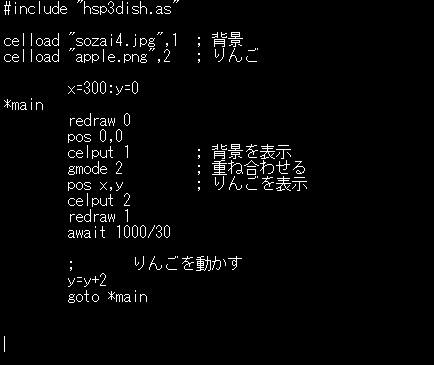
\includegraphics[keepaspectratio,width=10.954cm,height=9.213cm]{text04-img/s_fallsrc.png}
    \end{center}
    \label{fig:prog_menu}
\end{figure}

変数xとyが、横と縦の位置を記憶していることはわかりましたか。

「y=y+2」という計算で下に向かって絵が動いていきます。

もっと速く動かすにはどうすればいいでしょうか?

別な方向、たとえば左から右、下から上に動かす方法を考えてみましょう。


\begin{description}
    \item \textgt{\bf \ \ 例題4-6 答え}
\end{description}



変数xの値を計算で変えることで横方向に、変数yの値を計算で変えることで縦方向に動かすことができます。

たとえば、「x=x+2」は右に、「y=y-2」は上に動くことになります。

計算で使っている「2」という数字は、1つのコマで動く大きさになります。

この値を変えることで、動く速さも変わります。大きな数字で速い速度、小さな数字で遅くなることを確認してみましょう。

%1578








